
\item A transparent thin film of uniform thickness and refractive index \( n_1 = 1.4 \) is coated on the convex spherical surface of radius \( R \) at one end of a long solid glass cylinder of refractive index \( n_2 = 1.5 \), as shown in the figure. Rays of light parallel to the axis of the cylinder traversing through the film from air to glass get focused at distance \( f_1 \) from the film, while rays of light traversing from glass to air get focused at distance \( f_2 \) from the film. Then
    \begin{center}
        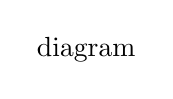
\begin{tikzpicture}
            \node at (0, 0) {diagram}; % Since I cannot draw the exact diagram, please replace "diagram.png" with the actual image path or extract the diagram using a drawing tool and insert it here.
        \end{tikzpicture}
    \end{center}
    \begin{tasks}(2)
        \task \( |f_1| = 3R \)
        \task \( |f_1| = 2.8R \)
        \task \( |f_2| = 2R \)\ans
        \task \( |f_2| = 1.4R \)
    \end{tasks}
